\documentclass{article}
\usepackage{xeCJK} 
\usepackage{amsmath}
\usepackage{amsfonts}
\usepackage{amssymb}
\usepackage{graphicx} % 引入图片宏包
\usepackage{tikz}

\setCJKmainfont{SimSun}

\usetikzlibrary{shapes.geometric, arrows}

\tikzstyle{startstop} = [rectangle, rounded corners, minimum width=3cm, minimum height=1cm, text centered, draw=black, fill=red!30]
\tikzstyle{process} = [rectangle, minimum width=3cm, minimum height=1cm, text centered, draw=black, fill=blue!20]
\tikzstyle{decision} = [diamond, minimum width=3.5cm, minimum height=1cm, text centered, draw=black, fill=green!20]
\tikzstyle{arrow} = [thick,->,>=stealth]

\begin{document}
\title{PRML第一次作业}
\author{许书闻 2023K8009926005}
\maketitle

\section{基于人脸识别的智能门禁系统}

\subsection{传感器:}
1.摄像头: 用于拍摄人脸图像\\
2. RFID读卡器: 用于读取ID卡信息作为辅助认证\\
3.红外传感器: 用于检测人员是否靠近门禁系统\\
\subsection{获取的数据:}
1.摄像头拍摄的人脸图像\\
2. RFID读卡器读取的ID卡信息\\
3.红外传感器检测到的人员信息\\
\subsection{进行的模式识别:}
1.人脸识别: 识别人脸图像中的人员身份\\
2. RFID认证: 读取ID卡信息,辅助人脸识别\\
3. 红外传感器: 检测人员是否靠近门禁系统\\
\subsection{结果和执行的操作:}
1.开门: 人员身份匹配成功,开门\\
2.记录日志: 记录人员进出门禁系统的时间\\
3.失败次数: 人员身份匹配失败,记录失败次数\\
4.触发警报: 失败次数达到一定阈值,触发警报,通知管理员\\

\subsection{处理流程:}
\begin{center}
    \begin{tikzpicture}[node distance=2cm]

        \node (start) [startstop] {开始:检测到人员};
        \node (capture) [process, below of=start] {摄像头拍摄人脸};
        \node (recognition) [process, below of=capture] {人脸识别 + RFID 认证};
        \node (decision) [decision, below of=recognition, yshift=-0.5cm] {身份匹配成功?};

        \node (open) [process, right of=decision, xshift=4.5cm] {开门 + 记录日志};
        \node (failcount) [process, below of=decision, yshift=-2.5cm] {失败次数 +1};
        \node (alarm) [process, below of=failcount, yshift=-2cm] {触发警报,通知管理员};
        \node (end) [startstop, below of=open, yshift=-3.5cm] {结束};

        \draw [arrow] (start) -- (capture);
        \draw [arrow] (capture) -- (recognition);
        \draw [arrow] (recognition) -- (decision);

        \draw [arrow] (decision.east) -- (open.west) node[midway, above] {是};
        \draw [arrow] (open.south) |- (end);
        \draw [arrow] (decision.south) -- (failcount.north) node[midway, right] {否};
        \draw [arrow] (failcount.south) -- (alarm.north);
        \draw [arrow] (alarm.south) |- (end);

    \end{tikzpicture}
\end{center}

\section{模式识别和机器学习的关系与区别}
\subsection{关系:}
模式识别(Pattern Recognition)和机器学习(Machine Learning, ML)密切相关,
机器学习是实现模式识别的重要方法。模式识别的目标是对输入数据进行分类或识别,
而机器学习提供了数据驱动的算法来自动学习模式和特征。
\subsection{机器学习方法的作用}
以人脸识别系统为例,机器学习在多个环节发挥关键作用:\\
1.数据采集:\\
\indent 通过摄像头等传感器获取人脸图像。\\
2.图像预处理:\\
\indent 归一化(Normalization)\\
\indent 去噪(Denoising)\\
\indent 直方图均衡化(Histogram Equalization)提高对比度\\
\indent → 机器学习可用于自适应调整图像质量,如 CNN 预处理模块。\\
3.特征提取:\\
\indent 传统方法:SIFT、HOG 特征\\
\indent 机器学习方法:深度学习 CNN 提取高维特征\\
4.模式分类:\\
\indent 传统方法:SVM、KNN 分类\\
\indent 机器学习方法:Softmax 分类、SVM 分类,或基于深度神经网络的端到端人脸识别(如 FaceNet、ArcFace)
5.结果匹配:\\
\indent 传统方法:基于特征距离的匹配\\  
\indent 机器学习方法:基于神经网络的匹配(如 FaceNet、ArcFace)\\
6.度量学习:\\
\indent 使用 度量学习(Metric Learning) 计算人脸特征的相似度。\\
7.执行决策:\\
\indent 根据人脸识别结果和 RFID\\
\indent 认证成功或失败,并执行相应操作(如解锁、门禁控制等)\\

\section{训练样本数、模型复杂度对经验误差和泛化性能的影响}
\subsection{训练样本数:}
\begin{itemize}
    \item 模型复杂度不变,训练样本数增加,通常导致经验误差减小;减小的幅度会逐渐趋缓,直到达到某个点后不再显著变化。
    \item 模型复杂度不变,训练样本数增加,泛化性能通常会提高,因为更多的样本能够帮助模型更好地理解数据的真实分布,减少过拟合的风险。
\end{itemize}

\subsection{模型复杂度:}
\begin{itemize}
    \item 训练样本数不变,模型复杂度增加会减小经验误差,但只有在模型复杂度适中时,经验误差才会有效减小;如果模型过于复杂,经验误差虽然会降低,但由于过拟合,泛化能力差,泛化误差会增大,导致模型在测试数据上的表现变差。
    \item 训练样本数不变,随着模型复杂度增加,泛化性能通常会呈现先升后降的趋势,即存在一个最优的模型复杂度,使得泛化误差最小。
\end{itemize}

\begin{table}[ht]
    \centering
    \begin{tabular}{|c|c|c|}
    \hline
    \textbf{影响因素} & \textbf{训练样本数增加} & \textbf{模型复杂度增加} \\
    \hline
    \textbf{经验误差} & 减小并趋于稳定 & 减小(对训练数据拟合程度升高) \\
    \hline
    \textbf{泛化性能} & 通常提高 & 适度复杂度提高,过度复杂导致过拟合 \\
    \hline
    \end{tabular}
    \caption{训练样本数与模型复杂度对经验误差和泛化性能的影响}
\end{table}    
\section{}
\subsection{(1)模式分类器为什么要进行模型选择?}
答:模式分类器进行模型选择的目的是为了在训练数据上获得最佳的拟合效果,同时保持较好的泛化性能。
\subsection{(2)模型参数和超参数}
答:模型参数是指模型内部的参数,通过训练数据学习得到,如线性回归中的权重和偏置。模型训练的目标就是调整这些参数,使模型在训练集上表现尽可能好。\\
超参数是指模型外部的参数,需要手动设置,如学习率、正则化系数等。超参数影响模型的训练过程,但不会被训练算法直接优化。\\
\begin{table}[ht]
    \centering
    \begin{tabular}{|c|c|c|}
    \hline
    \textbf{特征} & \textbf{模型参数} & \textbf{超参数} \\
    \hline
    \textbf{定义} & 模型通过训练自动优化的参数 & 用户预设的参数,影响训练过程 \\
    \hline
    \textbf{更新} & 在训练过程中由学习算法自动更新 & 训练前手动设置,并不随训练更新 \\
    \hline
    \textbf{举例} & 线性回归中的回归系数、神经网络中的权重和偏置 & 学习率、正则化系数、批量大小等 \\
    \hline
    \textbf{影响} & 直接影响模型的拟合能力和表现 & 影响模型的训练效率和最终性能 \\
    \hline
    \end{tabular}
    \caption{模型参数与超参数的比较}
\end{table}
    
模型参数和超参数的估计(以下方法由ChatGPT提供,整理下来供复习使用):\\

\subsection*{1. 模型参数的估计}

模型参数是通过训练算法自动优化的,它们直接影响模型的预测能力。一般来说,模型参数是通过学习算法在训练过程中估计的,具体方法取决于所使用的算法。以下是几种常见的模型参数估计方法:

\subsubsection*{(a) 线性回归中的参数估计}
在线性回归中,模型参数就是回归系数(权重)和截距。这些参数通过最小化均方误差(MSE)来进行估计。

\[\hat{\theta} = \arg\min_\theta \sum_{i=1}^n \left( y_i - \theta^T x_i \right)^2\]
其中,$y_i$ 是真实值,$x_i$ 是输入特征,$\theta$ 是需要优化的回归系数。

\subsubsection*{(b) 神经网络中的参数估计}
在神经网络中,模型参数主要是每层的权重和偏置。这些参数是通过反向传播(backpropagation)和优化算法(如梯度下降)来进行优化的。

\[
\theta_{t+1} = \theta_t - \eta \nabla_\theta L(\theta)
\]
其中,$L(\theta)$ 是损失函数,$\eta$ 是学习率,$\nabla_\theta L(\theta)$ 是损失函数关于参数的梯度。

\subsubsection*{(c) 支持向量机(SVM)中的参数估计}
在SVM中,模型参数是支持向量和超平面的权重。SVM通过最大化间隔来进行参数的优化。目标是通过求解以下凸优化问题来找到最佳的分割平面:

\[
\hat{w}, \hat{b} = \arg\min_{w,b} \frac{1}{2} \|w\|^2 \quad \text{subject to} \quad y_i (w^T x_i + b) \geq 1
\]
其中,$y_i$ 是样本的标签,$x_i$ 是输入特征,$w$ 和 $b$ 是需要优化的参数。

\subsection*{2. 超参数的估计}

与模型参数不同,超参数是在训练之前由用户指定的参数,它们影响模型的训练过程和性能。超参数的估计包括以下几种方法:

\subsubsection*{(a) 网格搜索(Grid Search)}
网格搜索是一种穷举式方法,通过遍历所有可能的超参数组合来找到最优的超参数设置。网格搜索的基本步骤包括:

\begin{enumerate}
    \item 定义一组可能的超参数值范围(如学习率、正则化系数等)。
    \item 枚举所有可能的超参数组合。
    \item 对每种超参数组合训练模型并计算其验证集上的表现(如准确率、F1分数等)。
    \item 选择使验证性能最好的超参数组合。
\end{enumerate}

\subsubsection*{(b) 随机搜索(Random Search)}
随机搜索是另一种优化方法,它不像网格搜索那样穷举所有可能的超参数组合,而是从定义的超参数空间中随机选择一定数量的组合进行评估。

\textbf{优点}:比网格搜索高效,尤其在高维超参数空间中,随机搜索通常能够更快地找到接近最优的超参数组合。

\subsubsection*{(c) 贝叶斯优化(Bayesian Optimization)}
贝叶斯优化是一种更智能的超参数优化方法,它通过建立一个**概率模型**来预测超参数对模型性能的影响,并基于这个模型选择下一个评估点。贝叶斯优化通过不断学习优化的过程,逐渐收敛到最优超参数。

\textbf{优点}:贝叶斯优化能够更有效地探索超参数空间,尤其适用于计算代价较高的模型。

\subsubsection*{(d) 交叉验证(Cross-validation)}
交叉验证是一种常用的验证方法,它可以用来评估超参数的效果。常见的方式是K折交叉验证,即将数据集分成 K 个子集,在每个子集上训练并验证模型,从而评估超参数的泛化性能。

例如,K折交叉验证中,超参数的选择通过评估在所有 K 折的平均验证误差来确定最优超参数。

\subsubsection*{(e) 超参数调优算法}
除了网格搜索、随机搜索和贝叶斯优化外,还可以使用一些其他的超参数调优算法,如遗传算法、粒子群优化等,这些算法能够通过模拟自然过程(如进化或群体行为)来搜索超参数空间。

\subsection{(3)M类的样本集的模型“训练-评价”过程}
答:对于M类的样本集,模型的“训练-评价”过程通常包括以下几个步骤:
\begin{enumerate}
    \item \textbf{数据准备}:将数据集分成训练集和测试集,通常采用交叉验证或留出法。
    \item \textbf{模型训练}:使用训练集对模型进行训练,学习样本的特征和类别之间的关系。
    \item \textbf{模型评价}:使用测试集对模型进行评价,计算模型在测试集上的性能指标,如准确率、精确率、召回率、F1分数等。
    \item \textbf{调参优化}:根据性能分析结果,对模型的超参数进行调优,以提高模型的泛化性能。    
    \item \textbf{反馈更新}:根据实际应用中的反馈信息,不断优化模型,提高模型的性能和适用性。
    \item \textbf{迭代训练}:根据新的数据和需求,不断迭代训练模型,使模型不断适应新的数据和场景。
\end{enumerate}

根据模型的训练效果、泛化能力、计算复杂度等方面综合考虑,最终选择最佳模型。可能还需要平衡模型的准确性和计算效率,选择合适的模型来部署。

\section{比较检验的目的和方法}
\subsection{比较检验的目的}
比较检验的目的是通过对不同模型、算法或参数设置的性能进行比较,找出最优的模型或参数设置,以提高模型的泛化性能和预测能力。
\subsection{比较检验的方法}
比较检验的方法包括以下几种:
\begin{enumerate}
    \item \textbf{二项检验(binomial test)}:目的是从测试错误率估计泛化错误率是否低于某阈值。
    \item \textbf{交叉验证(cross-validation)}:比较两个模型的泛化性能,找出最优模型。
    \item \textbf{t检验(t-test)}:用于估计平均测试错误率的置信度,比较两个样本均值之间的差异是否显著。
\end{enumerate}

\section{一个二分类问题的解}
\subsection{(1)Threshold=[0,0.2]时的Recall,Precision和F1}

\begin{figure}[h]
    \centering
    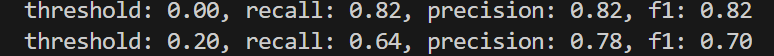
\includegraphics[width=0.8\textwidth]{Figure_2.png}
    \caption{各指标的值}
\end{figure}

\subsection{(2)等间距取[-1,1]内的15个值绘制ROC曲线}

\begin{figure}[h]
    \centering
    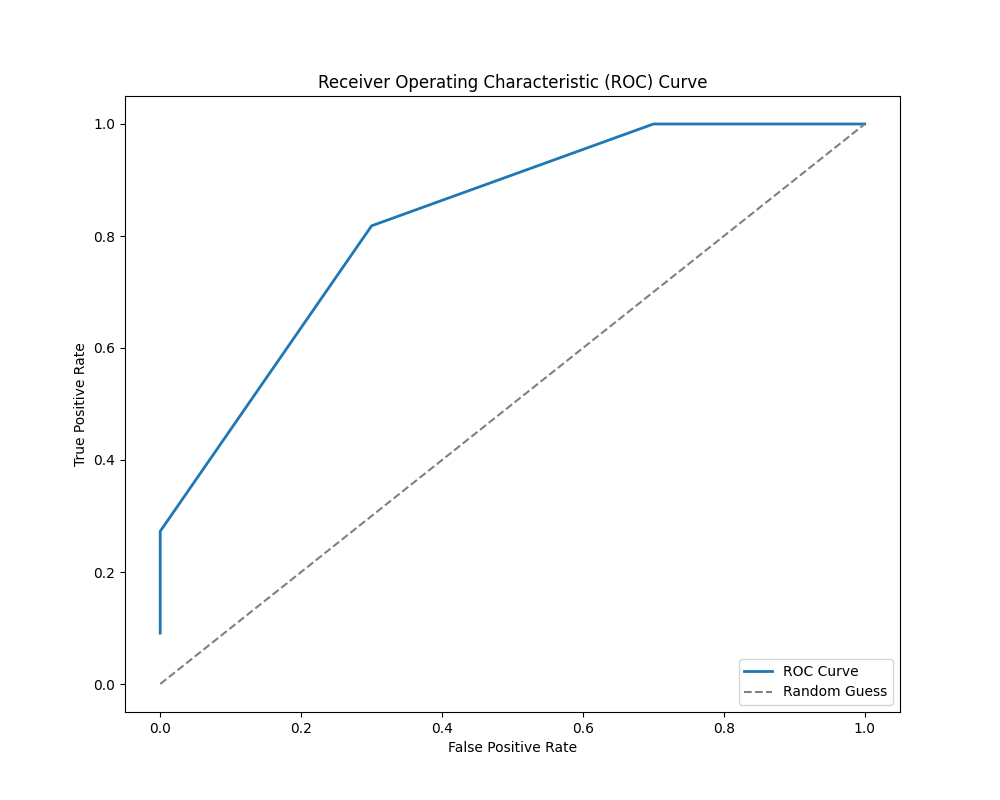
\includegraphics[width=0.6\textwidth]{Figure_1.png}
    \caption{$\theta_1=0.125,\theta_2=0.25$ 时的ROC曲线} % 图片标题
    \label{fig:example} % 交叉引用
\end{figure}
计算得到$AUC=0.83$

\subsection{(3)优化模型:}
1.令$\theta_2=0.25$,取:$\theta_1=[0.115,0.12,0.125,0.13,0.135]$计算得到$AUC=[0.90,0.88,0.83,0.77,0.71]$\\
2.令$\theta_1=0.125$,取:$\theta_2=[0.20,0.225,0.250,0.275,0.30]$计算得到$AUC=[0.818,0.823,0.827,0.832,0.827]$\\

可知若使$AUC$增大,$\theta_1$应减小,$\theta_2$应适当增大一点

\end{document}
